%%%%%%%%%%%%%%%%%%%%%%%%%%%%%%%%%%%%%%%%%%%%%%%%%%%%
\documentclass[12pt]{article}
\usepackage{sbc-template}
\usepackage{tikz}
\usepackage{listings}
\usepackage{color}

\newcommand{\mohammad}[1]{\textcolor{red}{Mohammad: #1}}

\definecolor{dkgreen}{rgb}{0,0.6,0}
\definecolor{gray}{rgb}{0.5,0.5,0.5}
\definecolor{mauve}{rgb}{0.58,0,0.82}
\lstset{frame=tb,
	language=Python,
	aboveskip=3mm,
	belowskip=3mm,
	showstringspaces=false,
	columns=flexible,
	basicstyle={\small\ttfamily},
	numbers=none,
	numberstyle=\tiny\color{gray},
	keywordstyle=\color{blue},
	commentstyle=\color{dkgreen},
	stringstyle=\color{mauve},
	breaklines=true,
	breakatwhitespace=true,
	tabsize=3
}
%%%%%%%%%%%%%%%%%%%%%%%%%%%%%%%%%%%%%%%%%%%%%%%%%%%%


%%%%%%%%%%%%%%%%%%%%%%%%%%%%%%%%%%%%%%%%%%%%%%%%%%%%
\title{Abstraction Layer for Data Cleaning Tools}
\author{Milad Abbaszadeh Jahromi\inst{1}, Mohammad Mahdavi\inst{1}, Ziawsch Abedjan\inst{1}}
\address{Technische Universit\"{a}t Berlin \email{\{milad.abbaszadehjahromi, mahdavilahijani, abdejan\}@tu-berlin.de}}
\begin{document} 
\maketitle
%%%%%%%%%%%%%%%%%%%%%%%%%%%%%%%%%%%%%%%%%%%%%%%%%%%%


%%%%%%%%%%%%%%%%%%%%%%%%%%%%%%%%%%%%%%%%%%%%%%%%%%%%
\begin{abstract} 
	Various data cleaning tools have been developed so far in data cleaning community. These tools are usually pointwise softwares that focus on specific types of data quality problems. Although combining these data cleaning tools together seems a promising idea, it is a hard task due to the heterogeneity of these tools. Each of these data cleaning tools has been written in different programming languages and has its own input/output format.
	
	In this document, we introduce our abstraction layer that hides these underlying heterogeneities from the user's application. The abstraction layer easily installs and configures the tools and provides fixed input/output system for running different data cleaning tools.
\end{abstract}
%%%%%%%%%%%%%%%%%%%%%%%%%%%%%%%%%%%%%%%%%%%%%%%%%%%%


%%%%%%%%%%%%%%%%%%%%%%%%%%%%%%%%%%%%%%%%%%%%%%%%%%%%
\section{Introduction}
\label{section:introduction}

\subsection{Motivation}
Data cleaning is the broad family of approaches that are aiming at improving data quality. There are different data cleaning tools that have been developed so far. Although combining these tools seems promising, heterogeneity and dispersion of these tools make it difficult to combine tools into one application. Each tool has been developed by a different people, in different programming languages. Furthermore, they usually have different installation processes and input/output systems. For a user that wants to combine these tools in a unique application, combining these heterogeneous data cleaning tools could be difficult, time consuming, and frustrating. 

In this document, we introduce our abstract layer that provides an easy-to-use framework for the user to work with different data cleaning tools. In particular, our abstraction layer provides simple APIs for installation of tools and running them on the datasets. 


\subsection{Contributions}
Our abstraction layer provides the following contributions:
\begin{itemize}
	\item Simple and guided process for installing different data cleaning tools.
	\item Easy-to-use framework to run different data cleaning tools by fixed input/output formats.
\end{itemize}


\subsection{Architecture}
Figure~\ref{figure:architecture} shows the position of the abstraction layer between the user's application and data cleaning tools. The user's application communicates with the abstraction layer in fixed input/output formats, regardless of the tool that application aims at running. Internally, the abstraction layer contains several wrappers for communicating with different data cleaning tools. Therefore, the heterogeneity of tools would be hidden for the user's application.

\begin{figure}[!h]
	\centering
	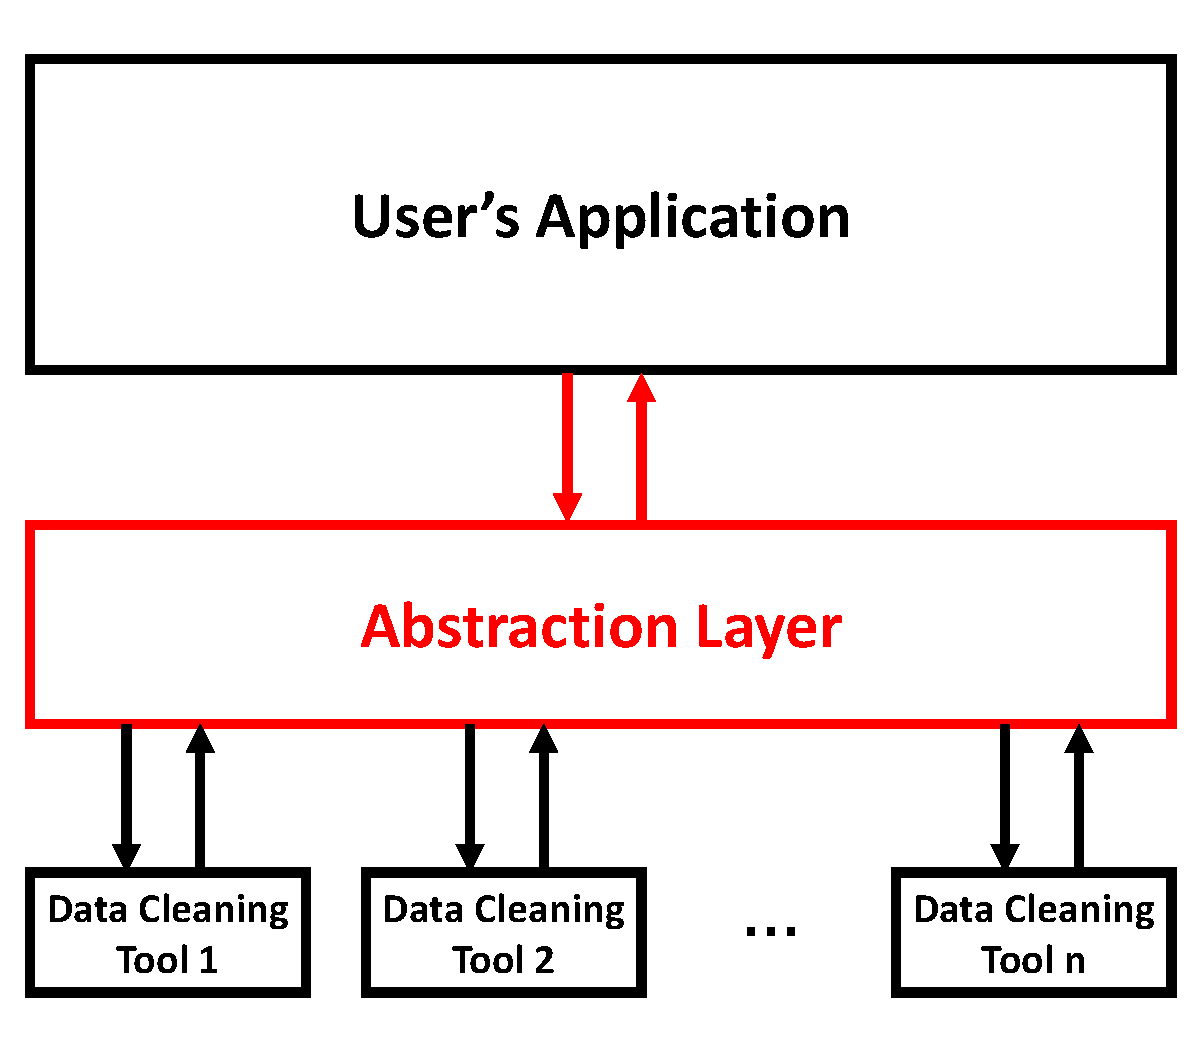
\includegraphics[scale=0.3]{attachments/architecture}
	\caption{The position of the abstraction layer between the user's application and data cleaning tools.}
	\label{figure:architecture}
\end{figure}


\subsection{Overview}
The rest of this document is organized as follows. In Section~\ref{section:installation}, we explain how the user can install the module. In Section~\ref{section:start_to_work}, we introduce the input/output format of the abstraction layer and provides some examples.
%%%%%%%%%%%%%%%%%%%%%%%%%%%%%%%%%%%%%%%%%%%%%%%%%%%%


%%%%%%%%%%%%%%%%%%%%%%%%%%%%%%%%%%%%%%%%%%%%%%%%%%%%
\section{Installation}
\label{section:installation}

\subsection{Prerequisites}
To install the module, you need first to install the followings:
\begin{itemize}
	\item Linux (Ubuntu/Debian recommended)
	\item Python 2.7
	\item Oracle Java 1.8
	\item Apache Ant 1.8.2+
	\item PostgreSQL 9.2+
\end{itemize}

\subsection{Setup}
After cloning the project, to install and configure the underlying data cleaning tools, it is enough to call the following API function:
\begin{lstlisting}
	install_tools()
\end{lstlisting}
This method installs and configures all the tools. 
%%%%%%%%%%%%%%%%%%%%%%%%%%%%%%%%%%%%%%%%%%%%%%%%%%%%


%%%%%%%%%%%%%%%%%%%%%%%%%%%%%%%%%%%%%%%%%%%%%%%%%%%%
\section{Start to Work}
\label{section:start_to_work}

To communicate to the abstraction layer, the user's application must call the following API function:
\begin{lstlisting}
	run_output = abstraction_layer(run_input)
\end{lstlisting}
This method takes a data cleaning job as input and returns the subsequent results as output. The formats of input/output objects are fixed. We explain these formats in the following subsections. 

\subsection{Input}
To call the abstraction layer, the user needs to provide a data cleaning job as input. This data cleaning job describe the data cleaning task that the abstraction layer should do for the user's application. The general template of the data cleaning job is as follows:
\begin{lstlisting}
	run_input = {
		"dataset": {
			"type": "dataset type",
			"param": ["list of parameters wrt. the dataset type"]
		},
		"tool": {
			"name": "tool name",
			"param": ["list of parameters wrt. the tool name"]
		}
	}
\end{lstlisting}
In practice, the data cleaning job is a JSON text that contains the following information: 
\begin{itemize}
	\item \textbf{dataset}. This part of the input configuration is responsible to describe the input dataset. It consists of two options.
	\begin{itemize}
		\item \textbf{type}. This option specifies the type of dataset. Currently, the module only supports \emph{csv} datasets.
		\item \textbf{param}. This option specifies the list of parameters that are needed for accessing the dataset. For csv datasets, this list contains only the path of dataset.
	\end{itemize}
	\item \textbf{tool}. The second part of the input configuration is responsible to describe the data cleaning tool that user aims at running on the input dataset. It consists of two options.
	\begin{itemize}
		\item\textbf{name}. This option specifies the name of the tool. Currently, the module supports \emph{dboost}~\cite{mariet2016outlier}, \emph{nadeef}~\cite{dallachiesa2013nadeef}, \emph{openrefine}~\cite{verborgh2013using}, and \emph{katara}~\cite{chu2015katara} tools.
		\item \textbf{param}. This option specifies the list of parameters that are needed for running the selected tool.		
	\end{itemize}

\end{itemize}

\paragraph{Example 1:} Running dBoost.
\begin{lstlisting}
	run_input = {
		"dataset": {
			"type": "csv",
			"param": ["datasets/sample.csv"]
		},
		"tool": {
			"name": "dboost",
			"param": ["gaussian", "1"]
		}
	}
\end{lstlisting}

\paragraph{Example 2:} Running NADEEF.
\begin{lstlisting}
	run_input = {
		"dataset": {
			"type": "csv",
			"param": ["datasets/sample.csv"]
		},
		"tool": {
			"name": "nadeef",
			"param": [["title", "brand_name"]]
		}
	}
\end{lstlisting}


\subsection{Output}
After calling the abstraction layer with proper input data cleaning job, it generates a list as output. This list consists of the cells in dataset, that have been marked as data errors along with the value that the data cleaning tool suggests as correction. The general template of the output list is as the follows:
\begin{lstlisting}
	run_output = [(i1, j1, v1), (i2, j2, v2),...]
\end{lstlisting}
Each element in the output list contains exactly three values referring to one specific cell in the dataset:
\begin{itemize}
	\item \textbf{Row number (i).} The row number of detected cell.
	\item \textbf{Column number (j)} The column number of detected cell.
	\item \textbf{Suggested value (v)}. The suggested value for this cell. 
\end{itemize}
%%%%%%%%%%%%%%%%%%%%%%%%%%%%%%%%%%%%%%%%%%%%%%%%%%%%


%%%%%%%%%%%%%%%%%%%%%%%%%%%%%%%%%%%%%%%%%%%%%%%%%%%%
\bibliographystyle{abbrv}
\bibliography{attachments/abbreviations,attachments/references}
\end{document}
%%%%%%%%%%%%%%%%%%%%%%%%%%%%%%%%%%%%%%%%%%%%%%%%%%%%